% Options for packages loaded elsewhere
\PassOptionsToPackage{unicode}{hyperref}
\PassOptionsToPackage{hyphens}{url}
%
\documentclass[
]{article}
\usepackage{amsmath,amssymb}
\usepackage{lmodern}
\usepackage{iftex}
\ifPDFTeX
  \usepackage[T1]{fontenc}
  \usepackage[utf8]{inputenc}
  \usepackage{textcomp} % provide euro and other symbols
\else % if luatex or xetex
  \usepackage{unicode-math}
  \defaultfontfeatures{Scale=MatchLowercase}
  \defaultfontfeatures[\rmfamily]{Ligatures=TeX,Scale=1}
\fi
% Use upquote if available, for straight quotes in verbatim environments
\IfFileExists{upquote.sty}{\usepackage{upquote}}{}
\IfFileExists{microtype.sty}{% use microtype if available
  \usepackage[]{microtype}
  \UseMicrotypeSet[protrusion]{basicmath} % disable protrusion for tt fonts
}{}
\makeatletter
\@ifundefined{KOMAClassName}{% if non-KOMA class
  \IfFileExists{parskip.sty}{%
    \usepackage{parskip}
  }{% else
    \setlength{\parindent}{0pt}
    \setlength{\parskip}{6pt plus 2pt minus 1pt}}
}{% if KOMA class
  \KOMAoptions{parskip=half}}
\makeatother
\usepackage{xcolor}
\IfFileExists{xurl.sty}{\usepackage{xurl}}{} % add URL line breaks if available
\IfFileExists{bookmark.sty}{\usepackage{bookmark}}{\usepackage{hyperref}}
\hypersetup{
  pdftitle={EviewsR: Seamless Integration of Eviews and R},
  pdfauthor={Sagiru Mati},
  hidelinks,
  pdfcreator={LaTeX via pandoc}}
\urlstyle{same} % disable monospaced font for URLs
\usepackage[margin=1in]{geometry}
\usepackage{color}
\usepackage{fancyvrb}
\newcommand{\VerbBar}{|}
\newcommand{\VERB}{\Verb[commandchars=\\\{\}]}
\DefineVerbatimEnvironment{Highlighting}{Verbatim}{commandchars=\\\{\}}
% Add ',fontsize=\small' for more characters per line
\usepackage{framed}
\definecolor{shadecolor}{RGB}{248,248,248}
\newenvironment{Shaded}{\begin{snugshade}}{\end{snugshade}}
\newcommand{\AlertTok}[1]{\textcolor[rgb]{0.94,0.16,0.16}{#1}}
\newcommand{\AnnotationTok}[1]{\textcolor[rgb]{0.56,0.35,0.01}{\textbf{\textit{#1}}}}
\newcommand{\AttributeTok}[1]{\textcolor[rgb]{0.77,0.63,0.00}{#1}}
\newcommand{\BaseNTok}[1]{\textcolor[rgb]{0.00,0.00,0.81}{#1}}
\newcommand{\BuiltInTok}[1]{#1}
\newcommand{\CharTok}[1]{\textcolor[rgb]{0.31,0.60,0.02}{#1}}
\newcommand{\CommentTok}[1]{\textcolor[rgb]{0.56,0.35,0.01}{\textit{#1}}}
\newcommand{\CommentVarTok}[1]{\textcolor[rgb]{0.56,0.35,0.01}{\textbf{\textit{#1}}}}
\newcommand{\ConstantTok}[1]{\textcolor[rgb]{0.00,0.00,0.00}{#1}}
\newcommand{\ControlFlowTok}[1]{\textcolor[rgb]{0.13,0.29,0.53}{\textbf{#1}}}
\newcommand{\DataTypeTok}[1]{\textcolor[rgb]{0.13,0.29,0.53}{#1}}
\newcommand{\DecValTok}[1]{\textcolor[rgb]{0.00,0.00,0.81}{#1}}
\newcommand{\DocumentationTok}[1]{\textcolor[rgb]{0.56,0.35,0.01}{\textbf{\textit{#1}}}}
\newcommand{\ErrorTok}[1]{\textcolor[rgb]{0.64,0.00,0.00}{\textbf{#1}}}
\newcommand{\ExtensionTok}[1]{#1}
\newcommand{\FloatTok}[1]{\textcolor[rgb]{0.00,0.00,0.81}{#1}}
\newcommand{\FunctionTok}[1]{\textcolor[rgb]{0.00,0.00,0.00}{#1}}
\newcommand{\ImportTok}[1]{#1}
\newcommand{\InformationTok}[1]{\textcolor[rgb]{0.56,0.35,0.01}{\textbf{\textit{#1}}}}
\newcommand{\KeywordTok}[1]{\textcolor[rgb]{0.13,0.29,0.53}{\textbf{#1}}}
\newcommand{\NormalTok}[1]{#1}
\newcommand{\OperatorTok}[1]{\textcolor[rgb]{0.81,0.36,0.00}{\textbf{#1}}}
\newcommand{\OtherTok}[1]{\textcolor[rgb]{0.56,0.35,0.01}{#1}}
\newcommand{\PreprocessorTok}[1]{\textcolor[rgb]{0.56,0.35,0.01}{\textit{#1}}}
\newcommand{\RegionMarkerTok}[1]{#1}
\newcommand{\SpecialCharTok}[1]{\textcolor[rgb]{0.00,0.00,0.00}{#1}}
\newcommand{\SpecialStringTok}[1]{\textcolor[rgb]{0.31,0.60,0.02}{#1}}
\newcommand{\StringTok}[1]{\textcolor[rgb]{0.31,0.60,0.02}{#1}}
\newcommand{\VariableTok}[1]{\textcolor[rgb]{0.00,0.00,0.00}{#1}}
\newcommand{\VerbatimStringTok}[1]{\textcolor[rgb]{0.31,0.60,0.02}{#1}}
\newcommand{\WarningTok}[1]{\textcolor[rgb]{0.56,0.35,0.01}{\textbf{\textit{#1}}}}
\usepackage{longtable,booktabs,array}
\usepackage{calc} % for calculating minipage widths
% Correct order of tables after \paragraph or \subparagraph
\usepackage{etoolbox}
\makeatletter
\patchcmd\longtable{\par}{\if@noskipsec\mbox{}\fi\par}{}{}
\makeatother
% Allow footnotes in longtable head/foot
\IfFileExists{footnotehyper.sty}{\usepackage{footnotehyper}}{\usepackage{footnote}}
\makesavenoteenv{longtable}
\usepackage{graphicx}
\makeatletter
\def\maxwidth{\ifdim\Gin@nat@width>\linewidth\linewidth\else\Gin@nat@width\fi}
\def\maxheight{\ifdim\Gin@nat@height>\textheight\textheight\else\Gin@nat@height\fi}
\makeatother
% Scale images if necessary, so that they will not overflow the page
% margins by default, and it is still possible to overwrite the defaults
% using explicit options in \includegraphics[width, height, ...]{}
\setkeys{Gin}{width=\maxwidth,height=\maxheight,keepaspectratio}
% Set default figure placement to htbp
\makeatletter
\def\fps@figure{htbp}
\makeatother
\setlength{\emergencystretch}{3em} % prevent overfull lines
\providecommand{\tightlist}{%
  \setlength{\itemsep}{0pt}\setlength{\parskip}{0pt}}
\setcounter{secnumdepth}{5}
\ifLuaTeX
  \usepackage{selnolig}  % disable illegal ligatures
\fi

\title{EviewsR: Seamless Integration of Eviews and R}
\author{Sagiru Mati}
\date{2022-07-06}

\begin{document}
\maketitle

{
\setcounter{tocdepth}{2}
\tableofcontents
}
\hypertarget{about-eviewsr}{%
\section{About EviewsR}\label{about-eviewsr}}

EviewsR is an R package that can run Eviews program from R. It also adds \texttt{eviews} as knit-engine to \texttt{knitr} package.

\hypertarget{installation}{%
\section{Installation}\label{installation}}

EviewsR can be installed using the following commands in R.

\begin{Shaded}
\begin{Highlighting}[]
\FunctionTok{install.packages}\NormalTok{(}\StringTok{"EviewsR"}\NormalTok{) }

\NormalTok{            OR}
            
\NormalTok{devtools}\SpecialCharTok{::}\FunctionTok{install\_github}\NormalTok{(}\StringTok{\textquotesingle{}sagirumati/EviewsR\textquotesingle{}}\NormalTok{)}
\end{Highlighting}
\end{Shaded}

\hypertarget{setup}{%
\section{Setup}\label{setup}}

To run the package successfully, you need to do one of the following

\begin{itemize}
\item
  Don't do anything if the name of EViews executable is one of the following: \texttt{EViews12\_x64}, \texttt{EViews12\_x86}, \texttt{EViews11\_x64}, \texttt{EViews11\_x86}, \texttt{EViews10}. The package will find the executable automatically.
\item
  Rename the Eviews executable to \texttt{eviews} or one of the names above.
\item
  Alternatively, you can use \texttt{set\_eviews\_path} function to set the path the EViews executable as follows:
\end{itemize}

\begin{Shaded}
\begin{Highlighting}[]
\FunctionTok{set\_eviews\_path}\NormalTok{(}\StringTok{"C:/Program Files (x86)/EViews 10/EViews10.exe"}\NormalTok{)}
\end{Highlighting}
\end{Shaded}

\hypertarget{usage}{%
\section{Usage}\label{usage}}

Please load the EviewsR package as follows:

\begin{verbatim}
```{r}                                                                .
library(EviewsR)
```
\end{verbatim}

\hypertarget{creating-a-workfile-from-r}{%
\section{Creating a workfile from R}\label{creating-a-workfile-from-r}}

An Eviews workfile can be created using \texttt{eviews\_wfcreate} function in R.

\begin{Shaded}
\begin{Highlighting}[]
\FunctionTok{eviews\_wfcreate}\NormalTok{(}\AttributeTok{wf=}\StringTok{"EviewsR\_workfile"}\NormalTok{,}\AttributeTok{page=}\StringTok{"EviewsR\_page"}\NormalTok{,}\AttributeTok{frequency =} \StringTok{"m"}\NormalTok{,}
\AttributeTok{start\_date =} \StringTok{"1990"}\NormalTok{,}\AttributeTok{end\_date =} \StringTok{"2022"}\NormalTok{)}
\end{Highlighting}
\end{Shaded}

\hypertarget{eviews-chunk}{%
\section{Eviews chunk}\label{eviews-chunk}}

A chunk for Eviews can be created by supplying \texttt{eviews} as the engine name as shown below:

\begin{verbatim}
```{eviews EviewsR,eval=T} 
    'This program is created in R Markdown with the help of EviewsR package
  
  wfcreate(page=EviewsR_page,wf=EviewsR_workfile) m 2000 2022
  for %y EviewsR package page1 page2
  pagecreate(page={%y}) EviewsR m 2000 2022
  next
  pageselect EviewsR_page
  rndseed 123456
  genr y=rnd
  genr x=rnd
  equation ols.ls y c x
  freeze(EviewsROLS,mode=overwrite) ols
  freeze(EviewsR_Plot,mode=overwrite) y.line
  wfsave EviewsR_workfile
```  
\end{verbatim}

\begin{Shaded}
\begin{Highlighting}[]
\NormalTok{    \textquotesingle{}This program is created in R Markdown with the help of EviewsR package}
  
\NormalTok{  wfcreate(page=EviewsR\_page,wf=EviewsR\_workfile) m 2000 2022}
\NormalTok{  for \%y EviewsR package page1 page2}
\NormalTok{  pagecreate(page=\{\%y\}) EviewsR m 2000 2022}
\NormalTok{  next}
\NormalTok{  pageselect EviewsR\_page}
\NormalTok{  rndseed 123456}
\NormalTok{  genr y=rnd}
\NormalTok{  genr x=rnd}
\NormalTok{  equation ols.ls y c x}
\NormalTok{  freeze(EviewsROLS,mode=overwrite) ols}
\NormalTok{  freeze(yy,mode=overwrite) y.line}
\NormalTok{  freeze(xx,mode=overwrite) x.line}
\NormalTok{  wfsave EviewsR\_workfile}
\end{Highlighting}
\end{Shaded}

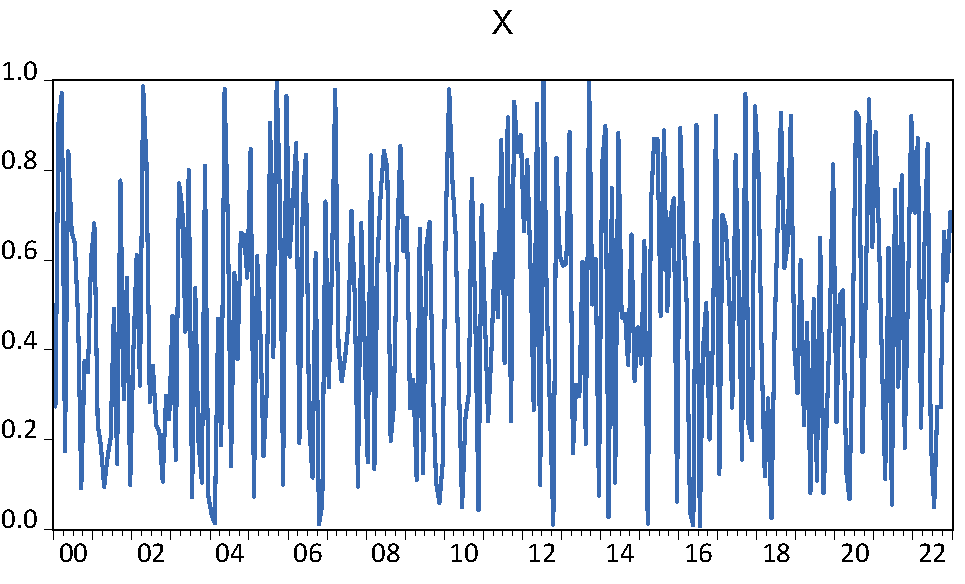
\includegraphics{eviewsr-eviewsr_page-xx.pdf} 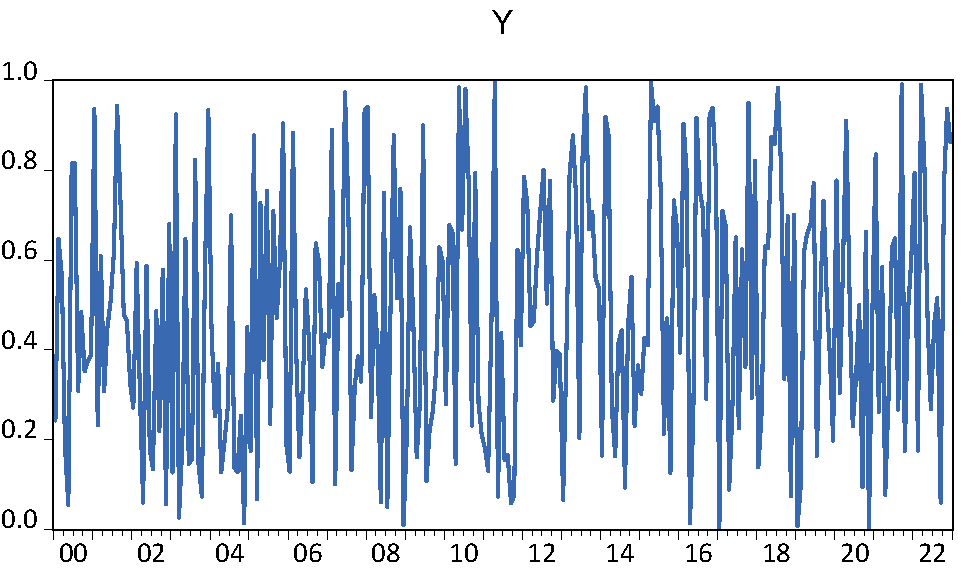
\includegraphics{eviewsr-eviewsr_page-yy.pdf}

The above chunk creates an Eviews program with the chunk's content, then automatically open Eviews and run the program, which will create an Eviews workfile with pages containing monthly sample from 2000 to 2022. The program will also save an Eviews workfile named \texttt{EviewsR} in the current directory.

The \texttt{eviews} chunk automatically returns the outputs of each equation object as a dataframe, accessible via \texttt{eviews\$equationName}. For example, The \(R^2\) of the \texttt{ols} equation object is , which can be accessed using \texttt{\textasciigrave{}r\ eviews\$ols\$r2{[}1{]}\textasciigrave{}}.

\hypertarget{executing-eviews-commands-in-r}{%
\section{Executing EViews commands in R}\label{executing-eviews-commands-in-r}}

A set of Eviews commands can be executed with the help of \texttt{exec\_commands} function in R. The above Eviews chunk can be translated using this function.

\begin{Shaded}
\begin{Highlighting}[]
\FunctionTok{exec\_commands}\NormalTok{(}\FunctionTok{c}\NormalTok{(}\StringTok{\textquotesingle{}wfcreate(page=EviewsR\_page,wf=EviewsR\_workfile) m 2000 2022\textquotesingle{}}\NormalTok{,}
  \StringTok{\textquotesingle{}for \%y EviewsR package page1 page2\textquotesingle{}}\NormalTok{,}
  \StringTok{\textquotesingle{}pagecreate(page=\{\%y\}) EviewsR m 2000 2022\textquotesingle{}}\NormalTok{,}
  \StringTok{\textquotesingle{}next\textquotesingle{}}\NormalTok{,}
\StringTok{\textquotesingle{}  pageselect EviewsR\_page\textquotesingle{}}\NormalTok{,}
  \StringTok{\textquotesingle{}rndseed 123456\textquotesingle{}}\NormalTok{,}
\StringTok{\textquotesingle{}  genr y=rnd\textquotesingle{}}\NormalTok{,}
  \StringTok{\textquotesingle{}genr x=rnd\textquotesingle{}}\NormalTok{,}
  \StringTok{\textquotesingle{}equation ols.ls y c x\textquotesingle{}}\NormalTok{,}
  \StringTok{\textquotesingle{}freeze(EviewsROLS,mode=overwrite) ols\textquotesingle{}}\NormalTok{,}
  \StringTok{\textquotesingle{}freeze(EviewsR\_Plot,mode=overwrite) y.line\textquotesingle{}}\NormalTok{,}
  \StringTok{\textquotesingle{}wfsave EviewsR\_workfile\textquotesingle{}}\NormalTok{,}
  \StringTok{\textquotesingle{}exit\textquotesingle{}}\NormalTok{))}
\end{Highlighting}
\end{Shaded}

\hypertarget{simulation-of-random-walk}{%
\section{Simulation of random walk}\label{simulation-of-random-walk}}

A set of random walk series can be simulated in R using EViews engine, thanks to \texttt{rwalk} function.

\begin{Shaded}
\begin{Highlighting}[]
\FunctionTok{rwalk}\NormalTok{(}\AttributeTok{wf=}\StringTok{"eviewsr\_workfile"}\NormalTok{,}\AttributeTok{series=}\StringTok{"X Y Z"}\NormalTok{,}\AttributeTok{page=}\StringTok{""}\NormalTok{,}\AttributeTok{rndseed=}\DecValTok{12345}\NormalTok{,}\AttributeTok{frequency=}\StringTok{"M"}\NormalTok{,}\AttributeTok{num\_observations=}\DecValTok{100}\NormalTok{)}
\end{Highlighting}
\end{Shaded}

\hypertarget{creating-eviews-object}{%
\section{Creating EViews object}\label{creating-eviews-object}}

The function \texttt{create\_object} can be used to create an Eviews object in the existing EViews workfile.

\begin{Shaded}
\begin{Highlighting}[]
\FunctionTok{create\_object}\NormalTok{(}\AttributeTok{wf=}\StringTok{"EviewsR\_workfile"}\NormalTok{,}\AttributeTok{action=}\StringTok{"equation"}\NormalTok{,}\AttributeTok{action\_opt=}\StringTok{""}\NormalTok{,}\AttributeTok{object\_name=}\StringTok{"eviews\_equation"}\NormalTok{,}\AttributeTok{view\_or\_proc=}\StringTok{"ls"}\NormalTok{,}\AttributeTok{options\_list=}\StringTok{""}\NormalTok{,}\AttributeTok{arg\_list=}\StringTok{"y ar(1)"}\NormalTok{)}
\end{Highlighting}
\end{Shaded}

\hypertarget{importing-table-as-kable}{%
\section{Importing table as kable}\label{importing-table-as-kable}}

Eviews tables can be imported as \texttt{kable} object by \texttt{import\_table} function. Therefore, we can include the results of the OLS generated by the Eviews chunk using the following R chunk;

For the OLS result only:

\begin{Shaded}
\begin{Highlighting}[]
\CommentTok{\# options(knitr.kable.NA = \textquotesingle{}\textquotesingle{})}
\FunctionTok{import\_table}\NormalTok{(}\AttributeTok{wf=}\StringTok{"EViewsR\_workfile"}\NormalTok{,}\AttributeTok{page=}\StringTok{"EviewsR\_page"}\NormalTok{,}\AttributeTok{table\_name =} \StringTok{"EViewsrOLS"}\NormalTok{,}\AttributeTok{table\_range =} \StringTok{"r7c1:r10c5"}\NormalTok{,}\AttributeTok{digits=}\DecValTok{3}\NormalTok{)}
\end{Highlighting}
\end{Shaded}

\begin{tabular}{l|r|r|r|r}
\hline
Variable & Coefficient & Std. Error & t-Statistic & Prob.\\
\hline
C & 0.496 & 0.033 & 14.882 & 0.000\\
\hline
X & -0.033 & 0.059 & -0.559 & 0.577\\
\hline
\end{tabular}

\hypertarget{saving-eviews-workfile}{%
\section{Saving EViews workfile}\label{saving-eviews-workfile}}

An EViews workfile can be saved various output formats using \texttt{eviews\_wfsave} in function in R.

\begin{Shaded}
\begin{Highlighting}[]
\FunctionTok{eviews\_wfsave}\NormalTok{(}\AttributeTok{wf=}\StringTok{"eviewsr\_workfile"}\NormalTok{,}\AttributeTok{source\_description =} \StringTok{"EviewsR\_wfsave.csv"}\NormalTok{)}
\end{Highlighting}
\end{Shaded}

\hypertarget{saving-eviews-page}{%
\section{Saving EViews page}\label{saving-eviews-page}}

Similar to Eviews workfile, an Eviews page can be saved in various formats by \texttt{eviews\_pagesave} function.

\begin{Shaded}
\begin{Highlighting}[]
\FunctionTok{eviews\_pagesave}\NormalTok{(}\AttributeTok{wf=}\StringTok{"eviewsr\_workfile"}\NormalTok{,}\AttributeTok{source\_description =} \StringTok{"EviewsR\_pagesave.csv"}\NormalTok{,}\AttributeTok{drop\_list =} \StringTok{"y"}\NormalTok{)}
\end{Highlighting}
\end{Shaded}

\hypertarget{importing-data-to-eviews}{%
\section{Importing data to EViews}\label{importing-data-to-eviews}}

Data can be imported from external sources by \texttt{eviews\_import} function.

\begin{Shaded}
\begin{Highlighting}[]
\FunctionTok{eviews\_import}\NormalTok{(}\AttributeTok{wf=}\StringTok{"eviewsr\_workfile"}\NormalTok{,}\AttributeTok{source\_description =} \StringTok{"EviewsR\_pagesave.csv"}\NormalTok{)}
\end{Highlighting}
\end{Shaded}

\hypertarget{import-data-from-eviews}{%
\section{Import data from EViews}\label{import-data-from-eviews}}

Use \texttt{import} function to import data from EViews to R as a dataframe. The function creates a new environment \texttt{eviews}, whose objects can be accessed via \texttt{eviews\$object\_name}.

\begin{Shaded}
\begin{Highlighting}[]

\FunctionTok{import}\NormalTok{(}\AttributeTok{object\_name =} \StringTok{"import"}\NormalTok{,}\AttributeTok{wf=}\StringTok{"eviewsr\_workfile"}\NormalTok{,}\AttributeTok{keep\_list =} \FunctionTok{c}\NormalTok{(}\StringTok{"x"}\NormalTok{,}\StringTok{"y"}\NormalTok{))}
\FunctionTok{plot}\NormalTok{(eviews}\SpecialCharTok{$}\NormalTok{import}\SpecialCharTok{$}\NormalTok{y,}\AttributeTok{type=}\StringTok{"l"}\NormalTok{,}\AttributeTok{ylab=}\StringTok{"EviewsR"}\NormalTok{,}\AttributeTok{col=}\StringTok{"red"}\NormalTok{)}
\end{Highlighting}
\end{Shaded}

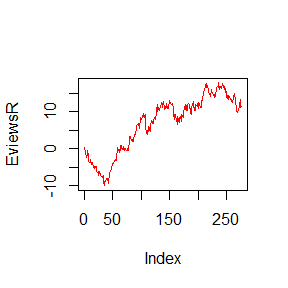
\includegraphics[width=1\linewidth,height=1\textheight]{EviewsR_files/figure-latex/import-1}

\hypertarget{exporting-dataframe-to-eviews}{%
\section{Exporting dataframe to EViews}\label{exporting-dataframe-to-eviews}}

Use \texttt{export} function to export dataframe object to Eviews.

\begin{Shaded}
\begin{Highlighting}[]
\FunctionTok{export}\NormalTok{(}\AttributeTok{wf=}\StringTok{"eviewr\_export"}\NormalTok{,}\AttributeTok{source\_description=}\NormalTok{eviews}\SpecialCharTok{$}\NormalTok{import,}\AttributeTok{start\_date =} \StringTok{\textquotesingle{}1990\textquotesingle{}}\NormalTok{,}\AttributeTok{frequency =} \StringTok{"m"}\NormalTok{)}
\end{Highlighting}
\end{Shaded}

\hypertarget{eviews-graph}{%
\section{EViews graph}\label{eviews-graph}}

EViews graph can be included in R Markdown or Quarto document by \texttt{eviews\_graph} function.

\begin{Shaded}
\begin{Highlighting}[]

\NormalTok{y}\OtherTok{=}\FunctionTok{runif}\NormalTok{(}\DecValTok{100}\NormalTok{)}
\NormalTok{x}\OtherTok{=}\FunctionTok{runif}\NormalTok{(}\DecValTok{100}\NormalTok{)}
\NormalTok{uu}\OtherTok{=}\FunctionTok{data.frame}\NormalTok{(x,y)}

 \FunctionTok{eviews\_graph}\NormalTok{(}\AttributeTok{wf=}\StringTok{"EviewsR\_workfile"}\NormalTok{,}\AttributeTok{page =} \StringTok{"EviewsR\_page"}\NormalTok{,}\AttributeTok{series=}\StringTok{"x y z"}\NormalTok{,}\AttributeTok{mode =} \StringTok{"overwrite"}\NormalTok{,}\AttributeTok{options =} \StringTok{"s"}\NormalTok{,}\AttributeTok{group =}\NormalTok{T)}
\CommentTok{\#\textgreater{} Warning in options$dev \textless{}{-} opts\_current$get("dev"): Coercing LHS to a list}
\end{Highlighting}
\end{Shaded}

\begin{figure}
\includegraphics[width=0.8\linewidth,height=0.8\textheight]{EviewsR_files/figure-latex//} \caption{EviewsR example figure}\label{fig:eviewsGraph}
\end{figure}

\begin{Shaded}
\begin{Highlighting}[]
 
  \CommentTok{\# eviews\_graph(wf="EviewsR\_workfile",page = "EviewsR\_page",series="x y",mode = "overwrite",options = "m",merge\_graphs =F,start\_date="1",frequency="5",save\_path = \textquotesingle{}\textquotesingle{})}
 
\end{Highlighting}
\end{Shaded}

\hypertarget{demo}{%
\section{Demo}\label{demo}}

The demo files are included and can be accessed via demo(package=``EviewsR'')

\begin{Shaded}
\begin{Highlighting}[]
\FunctionTok{demo}\NormalTok{(}\FunctionTok{create\_object}\NormalTok{())}
\CommentTok{\#\textgreater{} }
\CommentTok{\#\textgreater{} }
\CommentTok{\#\textgreater{}  demo(create\_object)}
\CommentTok{\#\textgreater{}  {-}{-}{-}{-} \textasciitilde{}\textasciitilde{}\textasciitilde{}\textasciitilde{}\textasciitilde{}\textasciitilde{}\textasciitilde{}\textasciitilde{}\textasciitilde{}\textasciitilde{}\textasciitilde{}\textasciitilde{}\textasciitilde{}}
\CommentTok{\#\textgreater{} }
\CommentTok{\#\textgreater{} \textgreater{} library(EviewsR)}
\CommentTok{\#\textgreater{} }
\CommentTok{\#\textgreater{} \textgreater{} demo(exec\_commands)}
\CommentTok{\#\textgreater{} }
\CommentTok{\#\textgreater{} }
\CommentTok{\#\textgreater{}  demo(exec\_commands)}
\CommentTok{\#\textgreater{}  {-}{-}{-}{-} \textasciitilde{}\textasciitilde{}\textasciitilde{}\textasciitilde{}\textasciitilde{}\textasciitilde{}\textasciitilde{}\textasciitilde{}\textasciitilde{}\textasciitilde{}\textasciitilde{}\textasciitilde{}\textasciitilde{}}
\CommentTok{\#\textgreater{} }
\CommentTok{\#\textgreater{} \textgreater{} library(EviewsR)}
\CommentTok{\#\textgreater{} }
\CommentTok{\#\textgreater{} \textgreater{} \# The first example creates an \textasciigrave{}EViews\textasciigrave{} workfile with monthly frequency from 1990 2021,}
\CommentTok{\#\textgreater{} \textgreater{} \# then save the workfile in the current working directory}
\CommentTok{\#\textgreater{} \textgreater{} }
\CommentTok{\#\textgreater{} \textgreater{} exec\_commands(c("wfcreate(wf=EviewsR\_exec\_commands,page=Page) m 2000 2022",}
\CommentTok{\#\textgreater{} +                 "save EviewsR\_exec\_commands","exit"))}
\CommentTok{\#\textgreater{} }
\CommentTok{\#\textgreater{} \textgreater{} \# The second example opens the \textasciigrave{}EViews\textasciigrave{} workfile and then generate a random series}
\CommentTok{\#\textgreater{} \textgreater{} \# named \textasciigrave{}y\textasciigrave{} and plots its line graph. It also freezes \textasciigrave{}ols\textasciigrave{} equation as \textasciigrave{}EviewsROLS\textasciigrave{}}
\CommentTok{\#\textgreater{} \textgreater{} }
\CommentTok{\#\textgreater{} \textgreater{} eviewsCommands=r\textquotesingle{}(genr y=rnd}
\CommentTok{\#\textgreater{} + genr x=rnd}
\CommentTok{\#\textgreater{} + equation ols.ls y c x}
\CommentTok{\#\textgreater{} + freeze(EviewsROLS,mode=overwrite) ols)\textquotesingle{}}
\CommentTok{\#\textgreater{} }
\CommentTok{\#\textgreater{} \textgreater{} exec\_commands(commands=eviewsCommands,wf="EviewsR\_exec\_commands")}
\CommentTok{\#\textgreater{} }
\CommentTok{\#\textgreater{} \textgreater{} \# unlink("EviewsR\_exec\_commands.wf1")}
\CommentTok{\#\textgreater{} }
\CommentTok{\#\textgreater{} \textgreater{} create\_object(wf="EviewsR\_exec\_commands",action="equation",action\_opt="",}
\CommentTok{\#\textgreater{} + object\_name="EviewsR\_create\_object",view\_or\_proc="ls",options\_list="",arg\_list="y ar(1)")}
\FunctionTok{demo}\NormalTok{(}\FunctionTok{eviews\_graph}\NormalTok{())}
\CommentTok{\#\textgreater{} }
\CommentTok{\#\textgreater{} }
\CommentTok{\#\textgreater{}  demo(eviews\_graph)}
\CommentTok{\#\textgreater{}  {-}{-}{-}{-} \textasciitilde{}\textasciitilde{}\textasciitilde{}\textasciitilde{}\textasciitilde{}\textasciitilde{}\textasciitilde{}\textasciitilde{}\textasciitilde{}\textasciitilde{}\textasciitilde{}\textasciitilde{}}
\CommentTok{\#\textgreater{} }
\CommentTok{\#\textgreater{} \textgreater{} library(EviewsR)}
\CommentTok{\#\textgreater{} }
\CommentTok{\#\textgreater{} \textgreater{} demo(exec\_commands)}
\CommentTok{\#\textgreater{} }
\CommentTok{\#\textgreater{} }
\CommentTok{\#\textgreater{}  demo(exec\_commands)}
\CommentTok{\#\textgreater{}  {-}{-}{-}{-} \textasciitilde{}\textasciitilde{}\textasciitilde{}\textasciitilde{}\textasciitilde{}\textasciitilde{}\textasciitilde{}\textasciitilde{}\textasciitilde{}\textasciitilde{}\textasciitilde{}\textasciitilde{}\textasciitilde{}}
\CommentTok{\#\textgreater{} }
\CommentTok{\#\textgreater{} \textgreater{} library(EviewsR)}
\CommentTok{\#\textgreater{} }
\CommentTok{\#\textgreater{} \textgreater{} \# The first example creates an \textasciigrave{}EViews\textasciigrave{} workfile with monthly frequency from 1990 2021,}
\CommentTok{\#\textgreater{} \textgreater{} \# then save the workfile in the current working directory}
\CommentTok{\#\textgreater{} \textgreater{} }
\CommentTok{\#\textgreater{} \textgreater{} exec\_commands(c("wfcreate(wf=EviewsR\_exec\_commands,page=Page) m 2000 2022",}
\CommentTok{\#\textgreater{} +                 "save EviewsR\_exec\_commands","exit"))}
\CommentTok{\#\textgreater{} }
\CommentTok{\#\textgreater{} \textgreater{} \# The second example opens the \textasciigrave{}EViews\textasciigrave{} workfile and then generate a random series}
\CommentTok{\#\textgreater{} \textgreater{} \# named \textasciigrave{}y\textasciigrave{} and plots its line graph. It also freezes \textasciigrave{}ols\textasciigrave{} equation as \textasciigrave{}EviewsROLS\textasciigrave{}}
\CommentTok{\#\textgreater{} \textgreater{} }
\CommentTok{\#\textgreater{} \textgreater{} eviewsCommands=r\textquotesingle{}(genr y=rnd}
\CommentTok{\#\textgreater{} + genr x=rnd}
\CommentTok{\#\textgreater{} + equation ols.ls y c x}
\CommentTok{\#\textgreater{} + freeze(EviewsROLS,mode=overwrite) ols)\textquotesingle{}}
\CommentTok{\#\textgreater{} }
\CommentTok{\#\textgreater{} \textgreater{} exec\_commands(commands=eviewsCommands,wf="EviewsR\_exec\_commands")}
\CommentTok{\#\textgreater{} }
\CommentTok{\#\textgreater{} \textgreater{} \# unlink("EviewsR\_exec\_commands.wf1")}
\CommentTok{\#\textgreater{} }
\CommentTok{\#\textgreater{} \textgreater{} eviews\_graph(wf="EviewsR\_exec\_commands",page = "page",series="x y",mode = "overwrite",options = "m")}
\CommentTok{\#\textgreater{} Warning in options$dev \textless{}{-} opts\_current$get("dev"): Coercing LHS to a list}
\CommentTok{\#\textgreater{} [1] "EviewsR\_files/figure{-}latex//"}
\CommentTok{\#\textgreater{} attr(,"class")}
\CommentTok{\#\textgreater{} [1] "knit\_image\_paths" "knit\_asis"}
\FunctionTok{demo}\NormalTok{(}\FunctionTok{eviews\_wfcreate}\NormalTok{())}
\CommentTok{\#\textgreater{} }
\CommentTok{\#\textgreater{} }
\CommentTok{\#\textgreater{}  demo(eviews\_wfcreate)}
\CommentTok{\#\textgreater{}  {-}{-}{-}{-} \textasciitilde{}\textasciitilde{}\textasciitilde{}\textasciitilde{}\textasciitilde{}\textasciitilde{}\textasciitilde{}\textasciitilde{}\textasciitilde{}\textasciitilde{}\textasciitilde{}\textasciitilde{}\textasciitilde{}\textasciitilde{}\textasciitilde{}}
\CommentTok{\#\textgreater{} }
\CommentTok{\#\textgreater{} \textgreater{} library(EviewsR)}
\CommentTok{\#\textgreater{} }
\CommentTok{\#\textgreater{} \textgreater{} eviews\_wfcreate(wf="EviewsR\_eviews\_wfcreate",page="EviewsR\_page",frequency = "m",}
\CommentTok{\#\textgreater{} +                 start\_date = "1990",end\_date = "2022")}
\end{Highlighting}
\end{Shaded}

\hypertarget{template}{%
\section{Template}\label{template}}

Template for R Markdown is created. Go to \texttt{file-\textgreater{}New\ File-\textgreater{}R\ Markdown-\textgreater{}\ From\ Template-\textgreater{}EviewsR}.

Please download the example files from \href{https://github.com/sagirumati/EviewsR/tree/master/inst/examples/}{Github}.

\end{document}
